\documentclass[conference]{IEEEtran}
\usepackage{graphicx}
\usepackage{booktabs}
\usepackage{url}
\usepackage{amsmath}
\usepackage{array}
\usepackage{xcolor}

\title{DT-RAM: A Shadow-Mode Edge--Cloud Resource-Management Prototype and Preliminary Telemetry Study}

\author{\IEEEauthorblockN{DT-RAM Project Team}}

\begin{document}
\maketitle

\begin{abstract}
Digital-twin-assisted reinforcement learning has been studied for edge offloading and network resource management, but a resource-management prototype must also connect telemetry, state handling, prediction, counterfactual evaluation, safety checks, and infrastructure control without confusing software checks with operational evidence. This paper documents DT-RAM, a modular prototype whose Python decision components are separated from a Go Kubernetes controller and whose current approval path is shadow-only. We report a provenance-recorded k3d integration capture and a preliminary comparison of seven CPU forecasting approaches on its idle telemetry. The capture contains 5,004 samples from three k3d nodes over approximately 30 minutes; the nodes share a Docker/WSL2 host, and the run contains no workload or fault injection. A temporal convolution has the lowest mean validation RMSE (0.013083 CPU-fraction units) among the evaluated models, while the interval coverage is unavailable because only three calibration residuals per model per horizon were retained. This short, autocorrelated capture does not establish distribution-free coverage. Its measured direct-inference p95 is 0.180 ms on the capture host. These results establish a narrow telemetry-pipeline and forecasting feasibility study. They do not establish independent node fidelity, forecasting under workload, benefit from reinforcement learning, or safe live actuation. The paper identifies the implementation and evidence needed to test those claims.
\end{abstract}

\begin{IEEEkeywords}
edge computing, digital twin, Kubernetes, resource management, forecasting, reinforcement learning, shadow mode
\end{IEEEkeywords}

\section{Introduction}
Resource management across cloud and edge clusters must balance utilization, service quality, and the cost of moving workloads. Digital twins and reinforcement learning have both been applied to related problems, including microservice offloading and network resource allocation \cite{chen2023,cheng2025}. The remaining engineering question for DT-RAM is narrower: how can telemetry and candidate decisions be routed through a prototype that preserves a controlled actuation boundary, and what evidence does its current testbed actually provide?

DT-RAM separates telemetry collection, twin state, forecasting, simulation, safety evaluation, and infrastructure control. Node.js services expose application-facing APIs; Go services collect telemetry and own Kubernetes access; Python services implement forecasting, simulation, and a PPO baseline scaffold. The gateway routes a candidate through simulation and the safety service, and the Go controller consumes approved shadow decisions. The code and deployment records show that this path is not yet a validated predictive control loop: simulation dynamics do not consume forecast values, the twin fidelity score remains zero in the documented k3d run, and the controller blocks live mutations.

This work therefore makes an implementation and measurement contribution with deliberately bounded claims. We document the prototype's service boundary and report a recorded telemetry integration and a forecasting comparison on an idle capture. The forecasting study uses causal contiguous windows, chronological partitions, common score origins, and a separate validation calibration procedure. It does not test an RL policy or compare resource-management outcomes. Prior research already studies DT-assisted RL for microservice offloading and resource allocation, Kubernetes digital twins, migration-cost-aware edge scheduling, and lightweight forecasting for orchestration \cite{chen2023,cheng2025,kubetwin2024,edgebus2024,aero2025}; DT--RL itself is not claimed as novel.

The specific contributions are:
\begin{itemize}
  \item We describe a modular, shadow-mode DT-RAM prototype and distinguish services exercised in the recorded k3d integration from services that remain scaffolded or unvalidated.
  \item We report a provenance-linked, 5,004-event idle k3d telemetry capture and its data-quality and fidelity limitations.
  \item We summarize a seven-model CPU forecast comparison and host-side inference measurements, explicitly treating unavailable calibration and non-workload telemetry as boundaries on the results.
\end{itemize}

\section{Related Work}
\textit{DT-assisted learning and resource decisions.} Chen \textit{et al.} combine digital-twin technology and deep reinforcement learning for resource-aware microservice offloading in collaborative edge computing \cite{chen2023}. Cheng \textit{et al.} describe DT-enhanced RL for network resource management and present case studies in wireless-network settings \cite{cheng2025}. These works rule out a broad novelty claim for combining DT and RL. DT-RAM's present evidence concerns service separation and a shadow-mode integration, not a new policy or a comparative resource-allocation result.

\textit{Cloud--edge twins and orchestration.} Bellavista \textit{et al.} implement and experimentally evaluate microservice and serverless digital-twin variants along the cloud--edge continuum \cite{bellavista2024}. KubeTwin studies digital twins for Kubernetes deployments at scale \cite{kubetwin2024}. Ranjbaran \textit{et al.} study online-learning-based digital-twin placement and re-placement across cloud and edge managers \cite{ranjbaran2024}; this concerns placement of the twin itself, a different decision from moving application workloads. EdgeBus combines Kubernetes-oriented co-simulation with migration-cost-aware container scheduling and a GKE-backed testbed evaluation \cite{edgebus2024}. These systems provide close context for DT-RAM's architecture and further limit claims that its modularity or migration-cost awareness alone is novel.

\textit{Forecasting for orchestration.} AERO evaluates lightweight forecasting with real cloud workload data, simulation, and live deployment for edge--cloud orchestration \cite{aero2025}. Its evaluation scope is substantially broader than DT-RAM's single idle CPU trace. Our model comparison is preliminary feasibility evidence and does not establish forecast superiority for orchestration. The closest defensible distinction is the specific provenance-recorded integration artifact and its observed limitations; broader novelty requires a systematic comparison of additional implementations and workload settings.

\section{System and Implementation}
\subsection{Service Boundary}
Fig.~\ref{fig:architecture} summarizes the implemented service roles. The telemetry agent publishes node metrics through NATS JetStream. The Go twin manager validates and stores timestamped node state, reports staleness, and optionally persists state to Redis. The prediction collector records telemetry in SQLite; the prediction API exposes read-only forecasts from an explicitly selected model. The gateway requests twin and prediction context, submits candidate actions to the simulation service, and sends safety context to the safety service. Approved shadow decisions are published to the Go infrastructure controller. PostgreSQL backs the experiment metadata service. Prometheus configuration and Kubernetes manifests are present; the documented testbed run deployed the Go telemetry/twin/controller services with NATS and Redis, not the complete Compose service graph.

\begin{figure}[t]
\centering
\fbox{\begin{minipage}{0.96\columnwidth}\centering
Telemetry agent (Go) $\rightarrow$ JetStream $\rightarrow$ Twin manager (Go)\\[2pt]
$\hspace{6pt}\downarrow$ read-only forecasts\hspace{50pt}$\downarrow$ twin state\\[-1pt]
Prediction (Python) $\rightarrow$ Gateway (TypeScript) $\rightarrow$ Simulation (Python)\\[2pt]
$\hspace{58pt}\downarrow$ candidate + evidence\\[-1pt]
Safety service (Python) $\rightarrow$ JetStream shadow decision $\rightarrow$ Go controller\\[2pt]
\textbf{Current boundary: controller dry-run; Kubernetes mutations blocked}
\end{minipage}}
\caption{DT-RAM service boundary as implemented. The arrows summarize interfaces; forecast values currently do not alter simulator dynamics.}
\label{fig:architecture}
\end{figure}

\subsection{Twin, Simulation, and Safety}
The Go twin manager validates CPU and memory utilization ranges, rejects older or future timestamps, and recomputes freshness on reads. A fidelity function compares physical samples against twin metrics, but a score is meaningful only when its physical reference is independent. The k3d capture did not provide a valid node-specific comparison because the agent measurements were host-scoped while metrics-server observations were node-specific.

The Python simulator accepts no-op, migration, placement, scaling, and resource-adjustment candidates. It applies illustrative CPU/memory capacity checks and fixed queueing-style latency and SLO-probability formulas; migration candidates receive estimated transfer cost and duration. The formulas are not calibrated against measured service latency or migration outcomes. The API accepts a prediction dictionary, but the simulator does not use forecast values in its state transitions or predicted resource dynamics. Thus the current implementation is a candidate-evaluation scaffold, not an empirically validated counterfactual digital twin.

The safety gate checks fidelity, prediction confidence, SLO risk, node health, destination CPU capacity, and in-process migration limits. The controller uses dry-run configuration, audits requests, and returns an unavailable response for live actions while authoritative evidence integration is pending. The controller's Kubernetes service account has scoped write permissions in the project namespace; the dry-run and code-level live-action block are therefore material controls. No Python component has a Kubernetes client path. Migration and placement execution, resource adjustment, durable audit, restart-safe idempotency, rollout verification, and rollback are not available.

\subsection{RL Status}
The RL service contains a Gymnasium environment and a Stable-Baselines3 PPO wrapper. The environment initializes a synthetic vector, but each transition updates only the first CPU value using a fixed action-specific adjustment. Actions do not select a workload or destination, most observation features do not evolve, and declared energy and cost weights are unused. PPO model training and performance evaluation are not represented in the recorded experiment artifacts. We therefore describe PPO as a baseline scaffold and do not report a trained policy or RL result.

\section{Forecasting Method}
\subsection{Telemetry and Sample Construction}
The prediction service consumes the implemented node metric event: timestamp, node ID, CPU and memory utilization fractions, and incoming/outgoing network throughput. Application request rate, latency, queue length, workload placement, and SLO labels are not present in the verified producer contract. The recorded analysis uses CPU utilization only.

Samples are bucketed at a one-second cadence. A forecast origin is retained only if all history buckets and all target buckets exist, so missing values are not imputed. The chronological split assigns windows by global time and keeps all target labels within their partition. The documented proportions are 60\% training, 20\% validation, and 20\% testing. The validation interval is divided into model-tuning, calibration, and coverage-audit regions with maximum-horizon guard gaps. Calibration and audit origins are spaced by at least the maximum horizon. Model comparison uses up to 64 evenly spaced common origins for tuning and test scores. The 5, 10, 30, and 60 second horizons share these settings.

Seven approaches are compared: persistence, ARIMA, ETS, LSTM, GRU, a compact temporal convolution, and a one-layer Transformer encoder. The 60-sample history setting yielded no valid windows on this gappy capture; the experiment explicitly used a 20-sample history. The temporal convolution was selected using mean validation RMSE. The test partition was not used for model selection. Metrics include MAE, RMSE, MAPE where defined, and $R^2$ where target variance is nonzero. Split-conformal-style residual radii are withheld when calibration counts do not support the requested finite-sample rank \cite{angelopoulos2023}. The autocorrelated trace and shared-host measurements do not establish exchangeability or a distribution-free coverage guarantee for this experiment.

\subsection{Benchmark Protocol}
The reported model benchmark measures mean per-forecast inference on the capture host. A separate 200-repeat benchmark reports direct inference and an in-process API measurement. The latter has no network hop, and these measurements do not represent a deployed edge device. The run records a dataset hash, source hash, Git commit, software versions, seed, and model configuration. The trace and trained weights are excluded from the checkout; the analysis names an external handoff bundle but provides no durable URL, which limits reproduction from this repository alone.

\section{Testbed and Results}
\subsection{Deployment Evidence}
The testbed report describes a local k3d cluster with one server and two agents on Docker Desktop Linux/WSL2, using K3s v1.32.5. Telemetry agents, twin manager, infrastructure controller, NATS, and Redis reached their recorded rollout checks. The collector stored observations for all three node IDs. The run was an idle baseline with no injected workload or fault, and physical actuation was disabled. A synthetic shadow-only scale request with zero reported fidelity was rejected (HTTP 422, not executed). This is evidence of pipeline integration and fail-closed rejection in that testbed, not of independent physical edge measurements or workload control.

The capture has 5,004 events (1,668 per node) from 2026-11-01 12:20:47 to 12:51:04 UTC. Each node has 1,662 occupied one-second buckets and 156 missing buckets within its span (8.58\%). The mean observed interval is 1.0899 seconds and the maximum gap is 9.557 seconds. The twin reported fidelity 0 for each node and autonomy disabled. All k3d nodes shared the host-level CPU and memory observations, which differed in measurement scope from metrics-server's per-node figures.

\subsection{CPU Forecast Comparison}
Table~\ref{tab:forecast} reports the four-horizon mean RMSE and the recorded mean per-forecast latency. RMSE is in CPU-utilization fraction units; lower is better. The temporal convolution has the best mean validation RMSE (0.013083), while GRU has the best mean test RMSE (0.016219). Selection remains based on validation data. The narrow test differences do not demonstrate a meaningful or statistically significant advantage. Most per-horizon $R^2$ values are near zero or negative. Each model has only three calibration residuals per horizon, so test interval coverage is unavailable and no model is recommended for activation.

\begin{table}[t]
\caption{Recorded CPU forecasting results. RMSE $\downarrow$ is the mean over 5/10/30/60 s horizons; latency is the recorded mean per forecast.}
\label{tab:forecast}
\centering
\footnotesize
\begin{tabular}{lrrr}
\toprule
Model & Val. RMSE $\downarrow$ & Test RMSE $\downarrow$ & Latency (ms) $\downarrow$\\
\midrule
Persistence & 0.017835 & 0.024384 & 0.0003\\
ARIMA & 0.014227 & 0.016786 & 13.6492\\
ETS & 0.014233 & 0.016760 & 2.3646\\
LSTM & 0.014385 & 0.016749 & 0.1560\\
GRU & 0.013712 & 0.016219 & 0.4126\\
Temporal convolution & \textbf{0.013083} & 0.016727 & \textbf{0.0691}\\
Transformer & 0.013857 & 0.016225 & 0.2415\\
\bottomrule
\end{tabular}
\end{table}

The temporal model's 200-repeat direct-inference p95 was 0.180 ms (mean 0.106 ms); its in-process API p95 was 16.199 ms (mean 12.824 ms). Its artifact was 5,021 bytes. These results meet the design's 100 ms software budget on the measured host but do not measure network latency, target-edge hardware, or deployed server resource use. Fig.~\ref{fig:metrics} shows the recorded per-horizon test metrics; the blank interval-coverage panel indicates unavailable coverage, not zero coverage.

\begin{figure}[t]
\centering
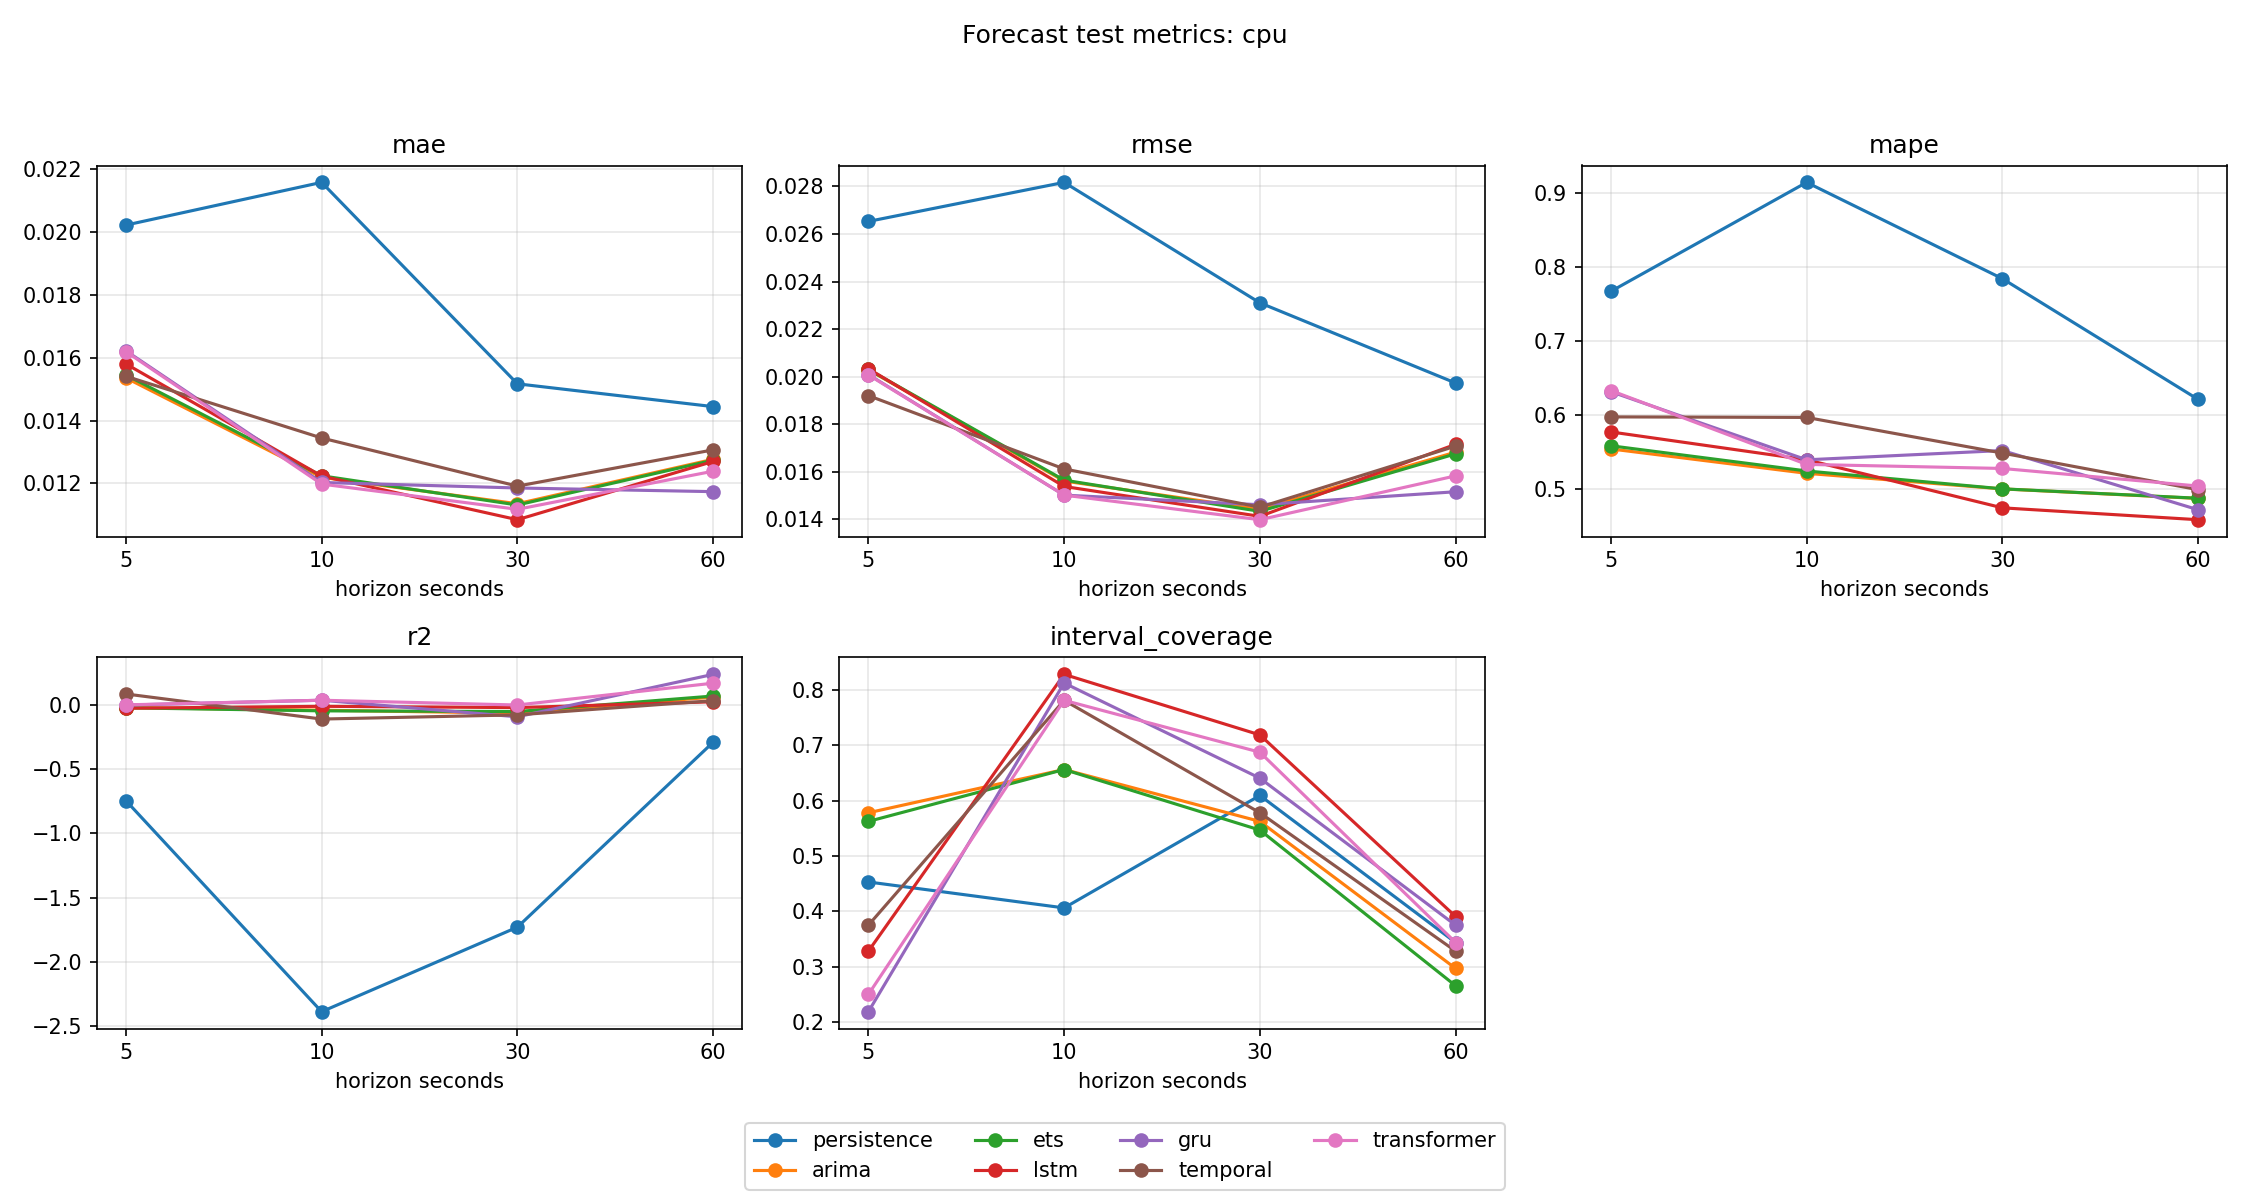
\includegraphics[width=\columnwidth]{../../experiments/analysis/k3d-20261101-forecasting/plots/metrics_cpu.png}
\caption{Per-horizon test metrics from the idle k3d CPU trace. Interval coverage is unavailable because calibration was insufficient.}
\label{fig:metrics}
\end{figure}

\section{Limitations and Discussion}
The evidence establishes that a telemetry event path can be deployed and recorded in a local k3d environment, that a low-fidelity shadow action can be rejected, and that seven forecasting implementations can be compared on a checksummed idle CPU trace. It does not show that the twin represents three independent nodes, that forecasts improve candidate evaluation, or that resource decisions improve application outcomes.

The experiment covers one short idle trace with substantial gaps and no workload, latency, request-rate, SLO, or fault labels. Dataset and model artifacts are not in the checkout, and the analysis depends on an external handoff bundle. The forecasting study has one dataset, one reported seed, and no repeated-run uncertainty analysis. The local-host latency benchmark cannot establish edge operational cost. The RL environment and simulator are simplified, forecasts do not affect simulator dynamics, and no trained PPO result or resource-management comparison exists. These are current technical limits on the claims, not merely deployment scope caveats.

The next research step is to collect a longer workload- and fault-labeled trace using node-specific measurements and application telemetry. The twin should then be validated against independent observations, and the simulator should be calibrated against measured resource, latency, and migration effects. Only after those steps can the project conduct reproducible heuristic-versus-PPO comparisons, DT/prediction/safety ablations, and controlled shadow-to-canary validation with durable audit and rollback. Until then, all approval remains shadow-only.

\section{Conclusion}
This paper documents DT-RAM as a modular shadow-mode prototype and reports a preliminary forecasting study on idle k3d telemetry. The telemetry capture and low-fidelity rejection provide evidence of a limited integration path; the temporal convolution yields the best validation RMSE in the recorded seven-model comparison, but interval coverage is unavailable and the trace does not represent independent workload-bearing edge nodes. The implementation does not yet demonstrate forecast-conditioned simulation, a validated PPO policy, or improved resource-management outcomes. Workload-aware measurement, twin/simulator validation, and controlled policy evaluation are necessary before those claims can be tested.

\bibliographystyle{IEEEtran}
\bibliography{references}
\end{document}
